\section{Proof Methods}

\frame{{Part 2: Proof Methods}

\tableofcontents[currentsection,hideallsubsections, firstsection=2, sections={2-4}]}

\subsection{Inference Rules}

\begin{frame}{Inference Rules}{}
  Inference (or logic deductions) are used to prove new propositions by using propositions that have been proposed before.
  \bigskip

  We normally write an inference as follows:

  \[
  \frac{P, Q, R}{X}
  \]

  This means "propositions P, Q, R are true, meaning that proposition X is true".\bigskip

  \structure{Inference Rules} are inferences that are particularly useful to build proofs. Let's see a few:
\end{frame}

\begin{frame}{Inference Rules}{Modus Ponens}
  The \emph{Modus Ponens} inference rule is:
  \[
  \frac{P, P\implies Q}{Q}
  \]
  If P is true, and P implies Q is true, then Q is true.\bigskip

  A few other related inference rules:
  \[
  \frac{P \implies Q, Q \implies R}{P \implies R},
  \frac{not(P) \implies not(Q)}{Q \implies P}
  \]

  So one way to prove a proposition is to {\bf start with propositions that you know are true} and {\bf use inference rules to reach the proposition you want to prove}.
\end{frame}

\subsection{Proving Implications}

\begin{frame}{Proving an Implication}{Direct Proof}
  The \emph{Modus Ponens} rule says that:
  \[
  \frac{P, P\implies Q}{Q}
  \]
  To prove $Q$, we have to prove that $P$, and that {\bf $P$ implies $Q$}.\bigskip

  We can prove an implication directly, by assuming $P$ is true, and showing that $Q$ must be true, step by step.\bigskip
\end{frame}

\begin{frame}{Proving an Implication}{Direct Proof}
{\bf Theorem:} If $0 \leq x \leq 2$, then $-x^3 + 4x + 1 > 0$\bigskip

\begin{proof}
\begin{itemize}
  \item Let's assume $0 \leq x \leq 2$
  \item We can rewrite $-x^3 + 4x$ as $x(2-x)(2+x)$
  \item If $0 \leq x \leq 2$, then $x$, $(2-x)$, $(2+x)$ are all positive.
  \item $x(2-x)(2+x) \geq 0$
  \item $x(2-x)(2+x) + 1 > 0$
  \item $-x^3 + 4x + 1 > 0$
\end{itemize}
\end{proof}

\end{frame}

\begin{frame}{Proving an Implication}{Contrapositive}
  Another way to prove an implication is to "prove the contrapositive". This means using the following inference rule:

  \[
    \frac{\text{NOT}(Q) \implies \text{NOT}(P)}{P \implies Q}
  \]

  So if we show that when Q is false, then P is always false, it is equivalent to show that when P is true, then Q is always true.
\end{frame}

\begin{frame}{Proving an Implication}{Contrapositive}
  {\bf Theorem:} if $r$ is irrational, then $\sqrt{r}$ is also irrational.

  \begin{proof}
    We prove the contrapositive: If $\sqrt{r}$ is rational, then $r$ is also rational.
    \begin{itemize}
      \item If $\sqrt{r}$ is rational, then $\sqrt{r}=\frac{m}{n}$.
      \item $m$ and $n$ are integers (definition of rational numbers)
      \item Square both sides: $r = \frac{m^2}{n^2}$.
      \item $m^2$ and $n^2$ are also integers, so $r$ is rational.
    \end{itemize}
  \end{proof}
\end{frame}



\begin{frame}{Proving "If and only If"}
  Remember that "If and only If" can be defined as:
  \[
  \frac{P\implies Q, Q \implies P}{P\iff Q}
  \]

  So to prove $P\iff Q$, we can first prove the implication from $P$ to $Q$, and then prove the implication from $Q$ to $P$.\bigskip

  This is useful to show equivalence between two mathematical statements.
\end{frame}


\subsection{Proof by Cases}

\begin{frame}[fragile]{Proof By Cases}{Example}

  Let's say you are refactoring code, and you want to profe that the two code samples below are equivalent. How would you do it?
  \vfill

  \begin{block}{Code 1}
\begin{verbatim}
If (X > 0 OR (X <= 0 AND Y > 100))
  print("Hello!")
\end{verbatim}
  \end{block}
  \begin{block}{Code 2}
\begin{verbatim}
If (X > 0 OR Y > 100)
  print("Hello!")
\end{verbatim}
  \end{block}
\end{frame}

\begin{frame}{Proof By Cases}{Definition}
  \structure{Proof By Cases}, is a proof technique that uses the idea of "divide and conquer".\vfill

  You break one complicated problem into easier, smaller sub-problems.
  \vfill

  \alert{Important!} When you create the cases, make sure that all possible cases are covered!
\end{frame}

\begin{frame}{Example: Friends and Strangers}

  {\bf Theorem:} In a group of 6 people, where {\bf every pair} is either a friend or a stranger, then we {\bf always} have at least a set of \structure{3 mutual friends} or a set of \alert{3 mutual strangers}.

  \begin{center}
    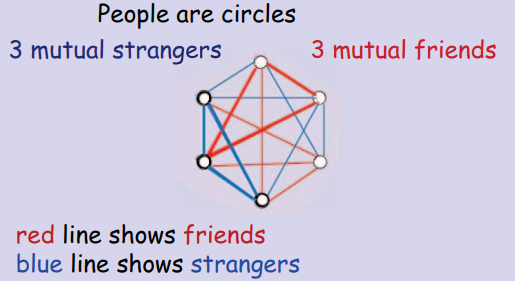
\includegraphics[width=0.8\textwidth]{../img/friends_and_strangers}
  \end{center}
\end{frame}

\begin{frame}{Example: Friends and Strangers}
  \begin{proof}
    The proof is by case analysis. Let "A" be one of the six people. There are two cases:
    \begin{enumerate}
      \item Among the 5 other people, at least 3 are friends with A;
      \item Among the 5 other people, at least 3 are strangers with A;
    \end{enumerate}\medskip

    Let's assume case (1). Let's call the three friends B, C, D. There are two subcases:
    \begin{enumerate}[A]
      \item B-C, C-D, or B-D are friends. We have now \structure{3 mutual friends} with A and the pair here.
      \item B-C, C-D and B-D are strangers. This makes a \structure{3 mutual strangers} set with the three pairs.
    \end{enumerate}\medskip

    This means that in case 1, the theorem holds. It is easy to see that case 2 is symmetrical to case 1.
  \end{proof}
\end{frame}


\begin{frame}{A WRONG Proof By Cases}

  {\bf Theorem:} $2a^2 > a$, for all $a\in \mathbb{Z}$.

  \begin{proof}
    The proof is by case analysis.
  \begin{enumerate}
    \item Case 1: $a > 0$;
    \begin{itemize}
      \item $2a^2$ is equal to $2a\times a$
      \item Since $a > 0$ and $a \in \mathbb{Z}$, then $a \geq 1$
      \item $2\times 1\times 1 > 1$
    \end{itemize}
    \item Case 2: $a < 0$
    \begin{itemize}
      \item Since $a < 0$ and $a \in \mathbb{Z}$, then $a \leq 1$
      \item For any negative $a$, $a^2$ is positive, so $a^2 > a$.
    \end{itemize}
    \end{enumerate}
    Because the theorem holds for case (1) and case (2), it holds for all possible cases.
  \end{proof}
  \bigskip

  What is wrong with this proof?
\end{frame}

\subsection{Proof by Contradiction}
\begin{frame}{Proof By Contradiction}{Definition}

  "Proof by Contradiction" is a technique where you show that {\bf the negative of the theorem implies a false fact to be true}.\bigskip

  For a simple example: "If gravity did not exist, then we would all be flying. Since we are not flying, then gravity must exist."\bigskip

  Sometimes, it can be easy to create a proof by contradiction by finding a good counter-example. Other times, we have to find an absurd consequence of the negative.\bigskip

  Use "Proof by Contradiction" to prove the following theorem:\\
  {\bf Theorem:} $\sqrt{2}$ is an irrational number.
\end{frame}


\begin{frame}{Proof by Contradiction}{Example}

  \begin{proof}
    We use proof by contradiction, and assume $\sqrt{2}$ is rational.
  \begin{enumerate}
  \item $\sqrt{2} = \frac{m}{n}$; $m,n \in \mathbb{Z}$; $n\neq 0$, and $m,n$ have no common factors.
  \item $n\sqrt{2} = m$ and squaring both sides give $2n^2 = m^2$.
  \item $m^2$ is even (because $n^2 = \frac{m^2}{2}$)
  \item If $m^2$ is even, then $m$ is even too. So $m = 2k$ for some integer $k$.
  \item So, $2n^2 = (2k)^2$, which leads to $n^2 = 2k^2$.
  \item Following the logic of (3) and (4), $n^2$ is even, and $n$ is even too.
  \item However, if $m$ and $n$ are even, it is a contradiction with (1).
  \end{enumerate}
  \end{proof}
\end{frame}



\subsection{The Well Ordering Outline}

\begin{frame}{Well Ordering Principle}{Definition}

  The Well Ordering Principle (WOP) is a very useful principle in mathematics, that can also look a little bit "obvious":\bigskip

  {\Large
  \begin{center}
    Every \structure{non-empty} set of\\
    \structure{Non-negative Integer Numbers} ($\mathbb{Z}^+$)\\
    has \alert{one smallest element}
  \end{center}}
\end{frame}

\begin{frame}{Well Ordering Principle}
  \frametitle{Well Ordering Examples}
    \begin{itemize}
      \item What is the smallest age among students in Tsukuba?
      \bigskip

      \item What is the smallest number of coins that adds to 876 yens?
      \bigskip

      \item What are the smallest integers $m$ and $n$ so that $x = \frac{m}{n}$?
    \end{itemize}
\end{frame}

\begin{frame}{Well Ordering Principle Proof Example}{}
  We can re-write the proof that $\sqrt{2}$ is irrational using WOP.

  \begin{proof}
  \begin{enumerate}
  \item $\sqrt{2} = \frac{m}{n}$; $m,n \in \mathbb{Z}$; $n\neq 0$;
  \item \alert{By WOP, there is a {\bf smallest} $m$ and $n$ so that $\sqrt{2} = \frac{m}{n}$}
  \item $n\sqrt{2} = m$ and squaring both sides give $2n^2 = m^2$.
  \item $m^2$ is even (because $n^2 = \frac{m^2}{2}$)
  \item If $m^2$ is even, then $m$ is even too. So $m = 2k$ for some integer $k$.
  \item So, $2n^2 = (2k)^2$, which leads to $n^2 = 2k^2$.
  \item Following the logic of (4) and (5), $n^2$ is even, and $n$ is even too.
  \item If $m$ and $n$ are even, then $\sqrt{2} = \frac{m/2}{n/2}$, and \alert{$m/2$, $n/2$ are smaller than $m,n$, contradicting the WOP}.
  \end{enumerate}
  \end{proof}
\end{frame}

\begin{frame}{Why is the WOP useful?}{General form for a WOP proof}

  The WOP gives us a general framework to produce proofs by contradiction:

  \begin{itemize}
    \item Structure your theorem around predicate $P(n)$, where $n \in \mathbb{N}$.
    \item Define a set $C$ of counter examples, so that $C ::=\{n \in \mathbb{N}| P(n) \text{ is false}\}$.
    \item By WOP, consider the minimum element $m \in C$.
    \item Find a contradiction, for example:
    \begin{itemize}
      \item if $m$ exists, then it implies in the existence of a smaller element $m' < m, m' \in C$.
      \item if $m$ exists, then actually $P(m)$ is true, and $m$ is not actually in $C$.
    \end{itemize}
    \item Therefore, the minimum element $m$ does not exist, the counter example set $C$ does not exist, and $P(n)$ is true for all $n$.
  \end{itemize}
\end{frame}

\begin{frame}{WOP Proof examples:}
  Let's see two quick examples of proofs using WOP. Try doing these two proofs by yourself first:
  \vfill

  \begin{itemize}
    \item {\bf Theorem:} Every $n > 1, n\in\mathbb{N}$ is a product of prime numbers.\bigskip

    \item {\bf Theorem:} For every $n\in\mathbb{N}$, $P(n): n+8 = 5a+3b; a,b \in\mathbb{N}$.\\(for every $n$, $n+8$ is composed of a sum of 3s and 5s)
  \end{itemize}
\end{frame}

\begin{frame}{WOP Proof example I: Prime factors}

  {\bf Theorem:} Every integers bigger than 1 is a product of prime numbers.
  \begin{proof}
    Proof by contradiction using the WOP.
    \begin{itemize}
      \item Assume, by WOP, that $m$ is the smallest $\mathbb{N}$ that is not a product of prime numbers.
      \item Obviously $m$ is not a prime, so $m = a_1a_2\ldots a_n$, where $a_i$ is not prime.
      \item Is $a_i$ a product of prime numbers?
      \begin{itemize}
        \item If $a_i$ is a product of prime numbers, then $a_i$ = $p_1p_2\ldots p_n$, and $m$ is now a product of prime numbers (\alert{contradiction})
        \item If $a_i$ is not a product of prime numbers, then $m$ is not the {\bf smallest} product of prime numbers. (\alert{contradiction})
      \end{itemize}
    \end{itemize}
  \end{proof}
\end{frame}

\begin{frame}{WOP Proof example II: Postal Numbers}
  {\bf Theorem:} For every $n$, $n+8$ is composed of 3s and 5s.

  \begin{proof}
    Proof by contradiction using the WOP
    \begin{itemize}
      \item First, we quickly verify that $P(n)$ is true for 0..8
      \item By WOP, we assume that there is some minimum $m > 8$ where $P(m)$ is false.
      \item If $P(m)$ is false, then $m+8$ cannot be composed of 3s and 5s.
      \item If $m$ is minimum, then $P(m-8)$ is true, and $m$ is composed of 3s and 5s.
      \item If $m$ is composed of 3s and 5s, then $m+8$ is $m+3+5$, and $P(m)$ is true! (\alert{Contradiction})
    \end{itemize}
  \end{proof}
\end{frame}
